\documentclass[11pt,a4paper]{article}
\usepackage[margin=2.3cm]{geometry}
\usepackage[T1]{fontenc}
\usepackage[utf8]{inputenc}
\usepackage{lmodern}
\usepackage{graphicx}
\usepackage{booktabs}
\usepackage{array}
\usepackage{caption}
\usepackage{float}
\usepackage[hidelinks]{hyperref}
\captionsetup{font=small,labelfont=bf}
\setlength{\parskip}{0.5em}
\setlength{\parindent}{0pt}
\renewcommand{\arraystretch}{1.12}

\title{\textbf{Supplementary Material 13}\\[0.3em]
\large Control theory analysis with gene expression at several correlation thresholds}
\author{\normalsize Supplement to the MRCONTROL article, PLOS Computational Biology (2025)\\
\normalsize doi:\href{https://doi.org/10.1371/journal.pcbi.1013725}{10.1371/journal.pcbi.1013725}}
\date{November 2026}

\begin{document}
\maketitle

\section{Purpose}

In the main article, the control theory step was applied to the directed human protein interaction (PPI) network of Vinayagam et al.\ \cite{vinayagam2011}. The gene expression file was used to identify the genes that were measured, and the expression values did not enter the network. The 16 network driver genes reported in the main article therefore describe the structure of the general human PPI network.

In this supplement we add the analysis in which gene expression is used. Specifically, an interaction is kept only when its two genes are correlated across patients, and the control theory analysis is repeated at several correlation thresholds. We report the genes that remain at every threshold (core genes) and the genes that change with the threshold. Moreover, we describe four controls that indicate how these gene lists should be interpreted. All tables and figures are produced by the script \texttt{Code/ControlTheory\_expression.R} of the repository.

\section{Data and method}

\textbf{Expression data.} We used the whole blood RNA sequencing data of GSE215865 \cite{thompson2023}, which were collected during the hospital stay for the acute infection. The Long COVID group has 155 patients with expression data and the recovered group has 27 patients, both defined with the checklist of Thompson et al.\ \cite{thompson2023}. Of the 155 patients with Long COVID, 152 belong to the 158 individuals analysed in the main article. For patients with several samples we used the median of each gene, which gives one value per patient and gene. The analysis includes 13,929 protein coding genes.

\textbf{Network.} The PPI network has 34,814 directed interactions, of which 25,211 have both genes measured (4,770 proteins).

\textbf{Correlation filter.} For each interaction we computed the Spearman correlation $r$ between its two genes across the patients of a group. An interaction was kept if $|r|$ was at least the threshold. We used the thresholds 0, 0.1, 0.2, 0.3, 0.4, 0.5 and 0.6, where the threshold 0 keeps every measured interaction.

\textbf{Control theory.} We applied structural controllability \cite{liu2011} to each network. The analysis gives the minimum number of driver nodes ($N_D$), which are the proteins that must receive an outside signal so that the whole network can be steered. Each protein is then described in two ways. Type I describes the effect of removing the protein \cite{vinayagam2016}: \emph{critical} if $N_D$ increases, \emph{redundant} if $N_D$ decreases, and \emph{ordinary} if $N_D$ does not change. Type II describes whether the protein is itself a driver node \cite{jia2013}: \emph{critical} if it belongs to every minimum set of driver nodes, \emph{redundant} if it belongs to none, and \emph{ordinary} if it belongs to some of them. As in the main article, the score of a protein is its number of connections ($K$) multiplied by a weight of 2 for Type I critical proteins, 1 for Type II critical proteins and 0 otherwise, and the 16 proteins with the highest score are reported.

\textbf{Software.} The analysis uses the R function \texttt{run\_control\_theory()} in \texttt{Code/control\_theory.R}. It is an independent implementation of the published definitions and does not require any other controllability software (Section~\ref{sec:validation}).

\section{Correlation distribution and thresholds}

Figure~\ref{fig:dist} shows the correlations of the 25,211 interactions in the Long COVID group. The median of $|r|$ is 0.22, indicating that a threshold of 0.2 keeps about half of the interactions. Table~\ref{tab:thresholds} and Figure~\ref{fig:size} show what each threshold keeps. The network decreases from 25,211 interactions at the threshold 0 to 2,074 at the threshold 0.6, and the share of driver nodes increases from 36\% to 47\%.

\begin{figure}[H]
\centering
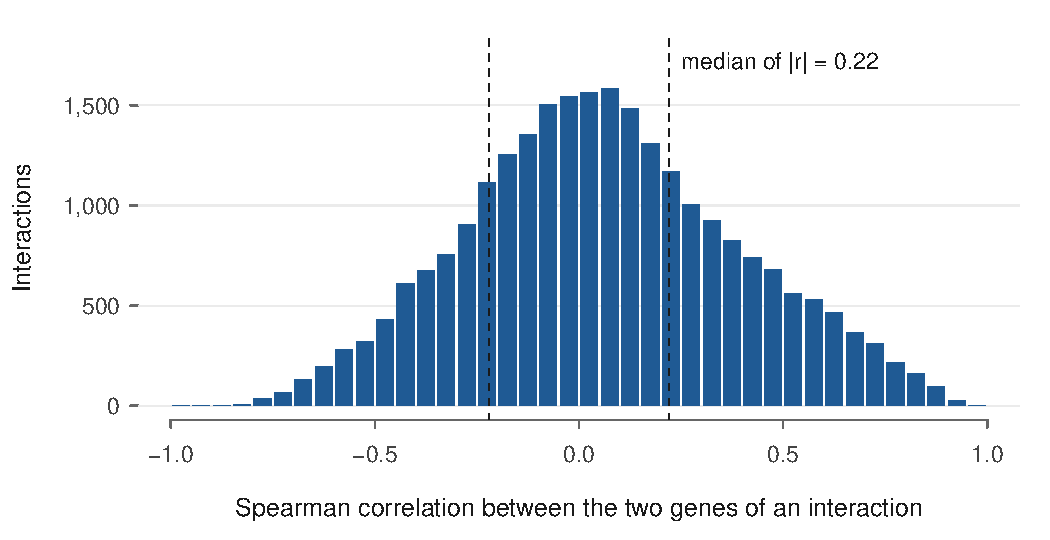
\includegraphics[width=0.82\textwidth]{figures/fig1_correlation_distribution.pdf}
\caption{Spearman correlation between the two genes of each PPI interaction in the Long COVID group (155 patients, 25,211 interactions). The dashed lines mark the median of $|r|$.}
\label{fig:dist}
\end{figure}

\begin{table}[H]
\centering
\caption{Networks of the Long COVID group at each correlation threshold. The share of interactions is relative to the 25,211 measured interactions. The share of driver nodes is relative to the proteins of that network.}
\label{tab:thresholds}
\small
\begin{tabular}{rrrrrrrrr}
\toprule
Threshold & \multicolumn{2}{c}{Interactions kept} & Proteins & \multicolumn{2}{c}{Driver nodes} & \multicolumn{3}{c}{Type I class} \\
\cmidrule(lr){2-3}\cmidrule(lr){5-6}\cmidrule(lr){7-9}
on $|r|$ & number & share & & number & share & critical & redundant & ordinary \\
\midrule
0.0 & 25,211 & 100\% & 4,770 & 1,740 & 36\% & 949 & 1,758 & 2,063 \\
0.1 & 19,010 & 75\% & 4,529 & 1,785 & 39\% & 848 & 1,761 & 1,920 \\
0.2 & 13,605 & 54\% & 4,108 & 1,747 & 43\% & 738 & 1,635 & 1,735 \\
0.3 & 9,409 & 37\% & 3,521 & 1,584 & 45\% & 606 & 1,389 & 1,526 \\
0.4 & 6,231 & 25\% & 2,759 & 1,253 & 45\% & 458 & 1,034 & 1,267 \\
0.5 & 3,769 & 15\% & 1,999 & 924 & 46\% & 337 & 693 & 969 \\
0.6 & 2,074 & 8\% & 1,309 & 614 & 47\% & 206 & 438 & 665 \\
\bottomrule
\end{tabular}

\end{table}

\begin{figure}[H]
\centering
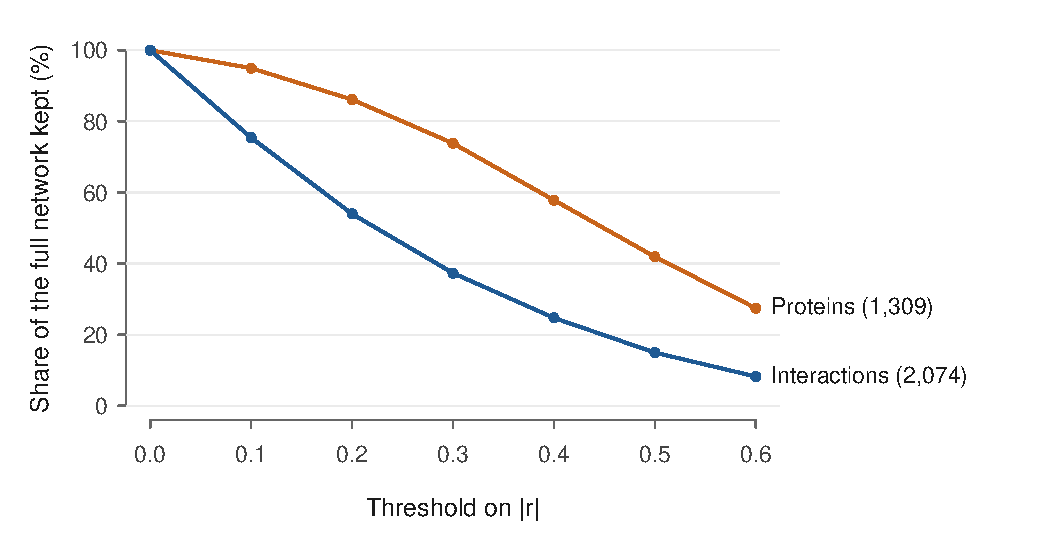
\includegraphics[width=0.82\textwidth]{figures/fig2_network_by_threshold.pdf}
\caption{Share of the interactions and of the proteins that remain in the Long COVID network at each threshold. The numbers at the right are the counts at the threshold 0.6.}
\label{fig:size}
\end{figure}

\section{Core genes and genes that change with the threshold}

Figure~\ref{fig:matrix} and Table~\ref{tab:top16} show the 16 genes with the highest score at each threshold in the Long COVID group. We distinguish three groups of genes.

\textbf{Core genes.} Six genes are in the top 16 at every threshold: TP53, EP300, CREBBP, GRB2, MAPK1 and FYN. All six belong to the 16 genes of the main article.

\textbf{Published genes that leave the top 16.} The other ten genes of the main article leave the top 16 as the threshold increases. Specifically, AR, CDKN1A and HDAC1 leave at the threshold 0.1, SRC and RB1 at 0.2, YWHAG and CSNK2A1 at 0.3, SMAD2 at 0.4, and SMAD3 and ESR1 at 0.5.

\textbf{Genes that enter the top 16.} Seventeen genes that are not among the 16 genes of the main article enter the top 16 at one or more thresholds (Table~\ref{tab:new}). GSK3B and LCK are present at six thresholds, SP1 at five and LYN at four. Several of these genes are kinases of immune cell signalling (LCK, LYN, HCK and SYK) or members of the JAK STAT pathway (STAT3 and JAK2).

The complete results for every gene and threshold, including the Type I and Type II classes, are in \texttt{tables/all\_genes\_by\_threshold\_LongCOVID.tsv}.

\begin{figure}[H]
\centering
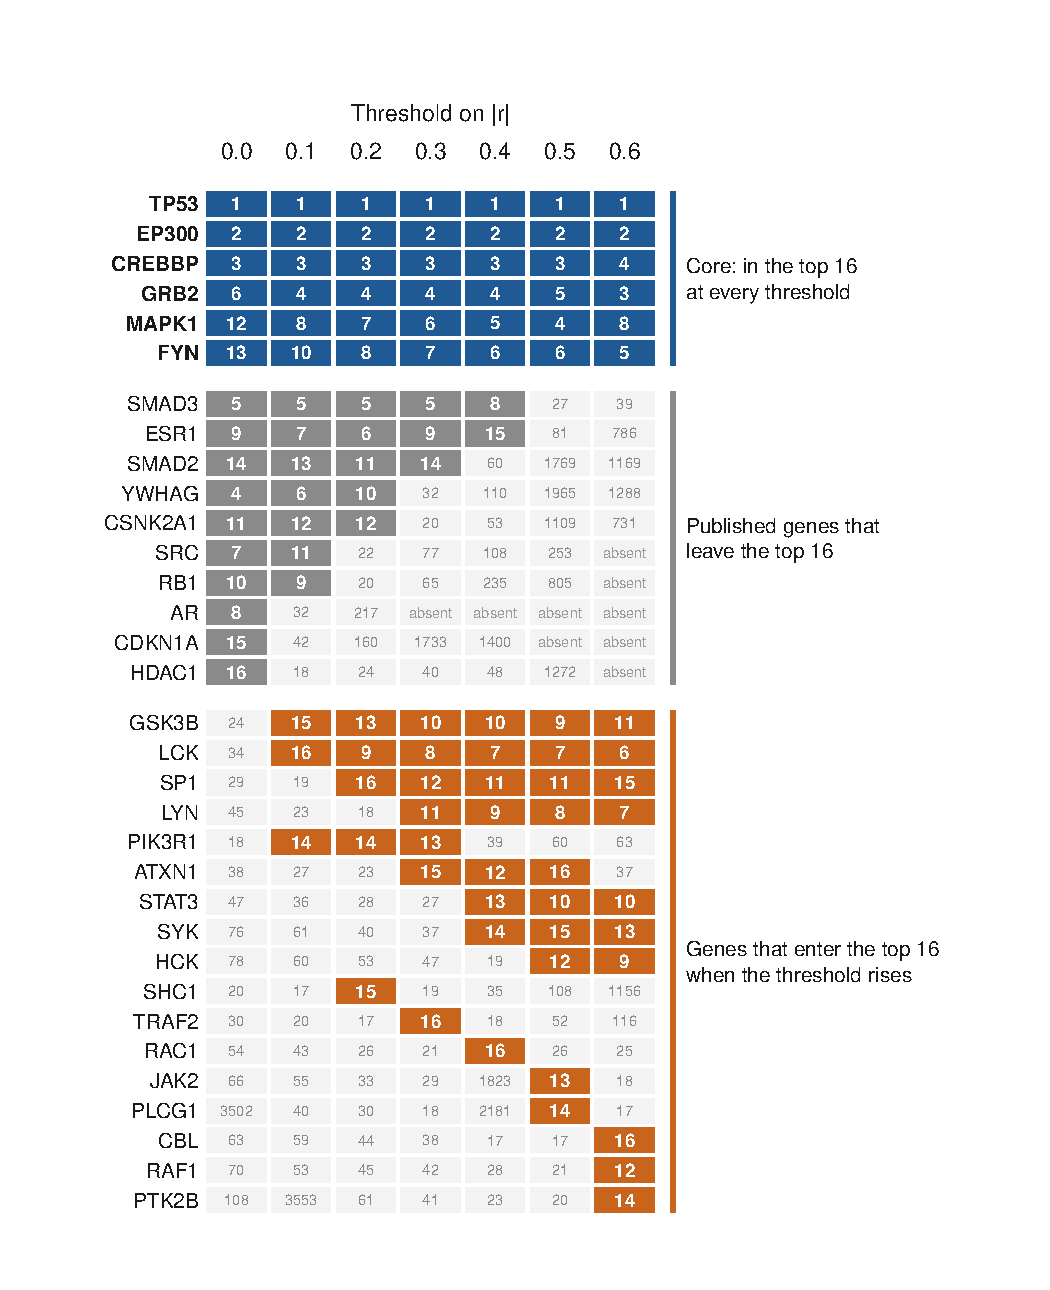
\includegraphics[width=0.74\textwidth]{figures/fig3_top16_across_thresholds.pdf}
\caption{Genes in the top 16 of the Long COVID group at any threshold. A filled cell indicates that the gene is in the top 16 at that threshold, and the number is its rank by score. Grey numbers are ranks outside the top 16. \emph{Absent} indicates that no interaction of the gene passes the threshold.}
\label{fig:matrix}
\end{figure}

\begin{table}[H]
\centering
\caption{The 16 genes with the highest score at each threshold in the Long COVID group. Bold: core genes. Italic with an asterisk: genes that are not among the 16 genes of the main article. \emph{Published}: number of the 16 genes of the main article in the list. \emph{Most connected}: number of the 16 genes that are also the 16 most connected proteins of that network.}
\label{tab:top16}
\footnotesize
\setlength{\tabcolsep}{3.5pt}
\begin{tabular}{r*{7}{l}}
\toprule
Rank & 0.0 & 0.1 & 0.2 & 0.3 & 0.4 & 0.5 & 0.6 \\
\midrule
1 & \textbf{TP53} & \textbf{TP53} & \textbf{TP53} & \textbf{TP53} & \textbf{TP53} & \textbf{TP53} & \textbf{TP53} \\
2 & \textbf{EP300} & \textbf{EP300} & \textbf{EP300} & \textbf{EP300} & \textbf{EP300} & \textbf{EP300} & \textbf{EP300} \\
3 & \textbf{CREBBP} & \textbf{CREBBP} & \textbf{CREBBP} & \textbf{CREBBP} & \textbf{CREBBP} & \textbf{CREBBP} & \textbf{GRB2} \\
4 & YWHAG & \textbf{GRB2} & \textbf{GRB2} & \textbf{GRB2} & \textbf{GRB2} & \textbf{MAPK1} & \textbf{CREBBP} \\
5 & SMAD3 & SMAD3 & SMAD3 & SMAD3 & \textbf{MAPK1} & \textbf{GRB2} & \textbf{FYN} \\
6 & \textbf{GRB2} & YWHAG & ESR1 & \textbf{MAPK1} & \textbf{FYN} & \textbf{FYN} & \textit{LCK}$^{\ast}$ \\
7 & SRC & ESR1 & \textbf{MAPK1} & \textbf{FYN} & \textit{LCK}$^{\ast}$ & \textit{LCK}$^{\ast}$ & \textit{LYN}$^{\ast}$ \\
8 & AR & \textbf{MAPK1} & \textbf{FYN} & \textit{LCK}$^{\ast}$ & SMAD3 & \textit{LYN}$^{\ast}$ & \textbf{MAPK1} \\
9 & ESR1 & RB1 & \textit{LCK}$^{\ast}$ & ESR1 & \textit{LYN}$^{\ast}$ & \textit{GSK3B}$^{\ast}$ & \textit{HCK}$^{\ast}$ \\
10 & RB1 & \textbf{FYN} & YWHAG & \textit{GSK3B}$^{\ast}$ & \textit{GSK3B}$^{\ast}$ & \textit{STAT3}$^{\ast}$ & \textit{STAT3}$^{\ast}$ \\
11 & CSNK2A1 & SRC & SMAD2 & \textit{LYN}$^{\ast}$ & \textit{SP1}$^{\ast}$ & \textit{SP1}$^{\ast}$ & \textit{GSK3B}$^{\ast}$ \\
12 & \textbf{MAPK1} & CSNK2A1 & CSNK2A1 & \textit{SP1}$^{\ast}$ & \textit{ATXN1}$^{\ast}$ & \textit{HCK}$^{\ast}$ & \textit{RAF1}$^{\ast}$ \\
13 & \textbf{FYN} & SMAD2 & \textit{GSK3B}$^{\ast}$ & \textit{PIK3R1}$^{\ast}$ & \textit{STAT3}$^{\ast}$ & \textit{JAK2}$^{\ast}$ & \textit{SYK}$^{\ast}$ \\
14 & SMAD2 & \textit{PIK3R1}$^{\ast}$ & \textit{PIK3R1}$^{\ast}$ & SMAD2 & \textit{SYK}$^{\ast}$ & \textit{PLCG1}$^{\ast}$ & \textit{PTK2B}$^{\ast}$ \\
15 & CDKN1A & \textit{GSK3B}$^{\ast}$ & \textit{SHC1}$^{\ast}$ & \textit{ATXN1}$^{\ast}$ & ESR1 & \textit{SYK}$^{\ast}$ & \textit{SP1}$^{\ast}$ \\
16 & HDAC1 & \textit{LCK}$^{\ast}$ & \textit{SP1}$^{\ast}$ & \textit{TRAF2}$^{\ast}$ & \textit{RAC1}$^{\ast}$ & \textit{ATXN1}$^{\ast}$ & \textit{CBL}$^{\ast}$ \\
\midrule
Published & 16 & 13 & 11 & 9 & 8 & 6 & 6 \\
Most connected & 16 & 16 & 16 & 16 & 16 & 16 & 16 \\
\bottomrule
\end{tabular}

\end{table}

\begin{table}[H]
\centering
\caption{Genes that enter the top 16 when the threshold increases. $K$ is the number of connections in the network with all measured interactions and in the network at the threshold 0.5. The known role is general background and is not a result of this analysis.}
\label{tab:new}
\footnotesize
\begin{tabular}{llrrp{7.4cm}}
\toprule
Gene & In the top 16 at & \multicolumn{2}{c}{Connections ($K$)} & Known role \\
\cmidrule(lr){3-4}
 & thresholds & all & at 0.5 & \\
\midrule
GSK3B & 0.1, 0.2, 0.3, 0.4, 0.5, 0.6 & 114 & 40 & Serine threonine kinase in WNT and insulin signalling \\
LCK & 0.1, 0.2, 0.3, 0.4, 0.5, 0.6 & 103 & 58 & Tyrosine kinase that starts T cell receptor signalling \\
SP1 & 0.2, 0.3, 0.4, 0.5, 0.6 & 109 & 38 & General transcription factor \\
LYN & 0.3, 0.4, 0.5, 0.6 & 94 & 51 & Src family kinase in B cell and myeloid cell signalling \\
PIK3R1 & 0.1, 0.2, 0.3 & 128 & 17 & Regulatory subunit of PI3 kinase \\
ATXN1 & 0.3, 0.4, 0.5 & 100 & 34 & Ataxin 1, a transcriptional regulator \\
STAT3 & 0.4, 0.5, 0.6 & 92 & 40 & Transcription factor activated by cytokines through JAK kinases \\
SYK & 0.4, 0.5, 0.6 & 72 & 35 & Tyrosine kinase downstream of B cell and Fc receptors \\
HCK & 0.5, 0.6 & 71 & 35 & Src family kinase of myeloid cells (monocytes, neutrophils) \\
SHC1 & 0.2 & 124 & 11 & Adaptor that links receptors to RAS MAPK signalling \\
TRAF2 & 0.3 & 108 & 19 & Adaptor in TNF receptor and NF kappa B signalling \\
RAC1 & 0.4 & 85 & 28 & Small GTPase that controls the cytoskeleton and cell movement \\
JAK2 & 0.5 & 77 & 35 & Kinase downstream of cytokine receptors (JAK STAT pathway) \\
PLCG1 & 0.5 & 87 & 35 & Phospholipase C gamma 1, downstream of T cell and growth factor receptors \\
CBL & 0.6 & 77 & 34 & E3 ubiquitin ligase that switches off tyrosine kinase signalling \\
RAF1 & 0.6 & 75 & 32 & Kinase of the RAS MAPK cascade \\
PTK2B & 0.6 & 62 & 32 & PYK2 tyrosine kinase, calcium dependent signalling in immune cells \\
\bottomrule
\end{tabular}

\end{table}

\section{How to read the gene lists: controls}

We ran four controls. Together they indicate that the lists above describe the PPI network after filtering with expression measured in patients with Long COVID, and that the present data do not show a difference from recovered patients.

\textbf{1. The ranking follows the number of connections.} At every threshold, the 16 genes with the highest score are the 16 most connected proteins of that network (Table~\ref{tab:top16}). The genes that enter the top 16 are therefore the highly connected proteins whose interactions pass the correlation filter.

\textbf{2. Interacting pairs and random pairs.} In whole blood, pairs of genes that do not interact are correlated almost as often as pairs that interact (Table~\ref{tab:controls}, Figure~\ref{fig:controls}a). At the threshold 0.3, 37.3\% of the PPI interactions pass, compared with 32.5\% of random pairs of the same genes. This suggests that the filter mainly reflects the general correlation structure of blood, for example the mixture of cell types, and only to a small extent the activity of specific interactions.

\textbf{3. Group size.} The recovered network is larger than the Long COVID network at every threshold. When 27 patients with Long COVID are drawn at random, their network has almost the same size as the recovered network (Table~\ref{tab:controls}, Figure~\ref{fig:controls}b). The difference in size is therefore explained by the number of patients.

\textbf{4. Long COVID compared with recovered patients.} The two groups share 10 to 14 of their top 16 genes at each threshold (Table~\ref{tab:controls}). We tested the differences between the groups by shuffling the group labels among the 182 patients while keeping the group sizes. The real groups do not differ more than the shuffled groups, in the control theory results and in the correlations themselves (Table~\ref{tab:shuffled}). After correction for multiple testing, no gene and no interaction differs between the groups.

\textbf{Interpretation.} The core genes are highly connected proteins of the human PPI network and remain central at every threshold. The genes in Table~\ref{tab:new} are candidates that may be of interest for further study in Long COVID, and they are not shown to be specific to Long COVID. Moreover, three limitations should be considered. The recovered group has only 27 patients, which allows only large differences to be detected. The samples were taken during the acute infection, before Long COVID developed. Finally, a correlation between two transcripts in whole blood does not demonstrate that the two proteins interact in the patients.

\begin{table}[H]
\centering
\caption{Controls 2 to 4. Random gene pairs: 300,000 pairs drawn from the same 4,770 genes. Long COVID (27 drawn): mean of 100 random draws of 27 patients.}
\label{tab:controls}
\small
\begin{tabular}{rrrrrrr}
\toprule
Threshold & \multicolumn{2}{c}{Pairs that pass (Long COVID)} & \multicolumn{3}{c}{Interactions in the network} & Shared genes \\
\cmidrule(lr){2-3}\cmidrule(lr){4-6}
 & PPI & random & Long COVID & Long COVID & recovered & in the top 16 \\
 & interactions & gene pairs & (155) & (27 drawn) & (27) & \\
\midrule
0.1 & 75.4\% & 72.8\% & 19,010 & 20,095 & 20,240 & 14 \\
0.2 & 54.0\% & 49.9\% & 13,605 & 15,301 & 15,522 & 12 \\
0.3 & 37.3\% & 32.5\% & 9,409 & 11,092 & 11,399 & 13 \\
0.4 & 24.7\% & 19.8\% & 6,231 & 7,602 & 7,967 & 10 \\
0.5 & 14.9\% & 10.8\% & 3,769 & 4,877 & 5,131 & 11 \\
0.6 & 8.2\% & 4.9\% & 2,074 & 2,814 & 3,012 & 12 \\
\bottomrule
\end{tabular}

\end{table}

\begin{figure}[H]
\centering
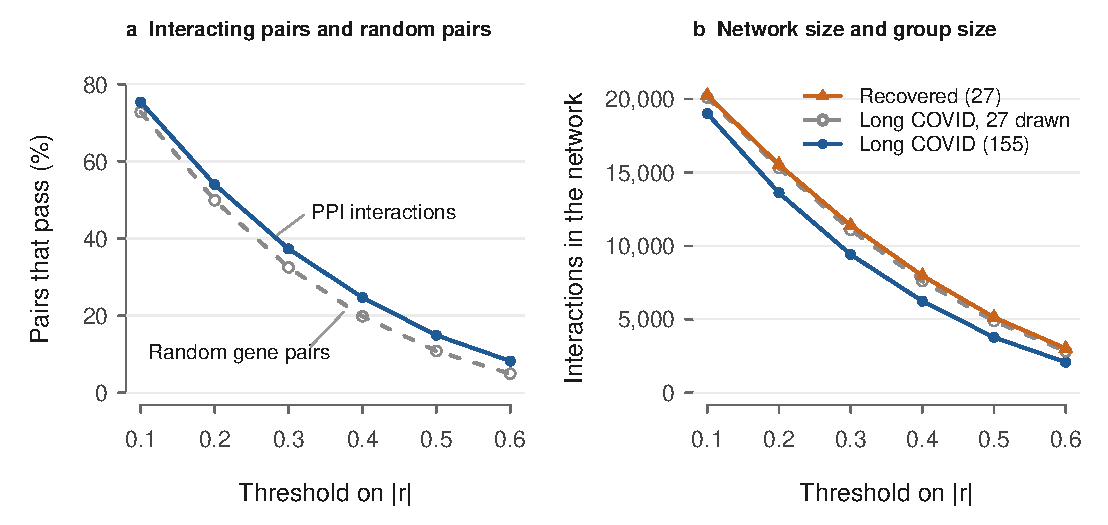
\includegraphics[width=0.95\textwidth]{figures/fig4_controls.pdf}
\caption{Controls. (a) Share of PPI interactions and of random gene pairs that pass each threshold in the Long COVID group. (b) Number of interactions in the network of each group.}
\label{fig:controls}
\end{figure}

\begin{table}[H]
\centering
\caption{Long COVID compared with recovered patients, with shuffled group labels (group sizes 155 and 27 kept). The last column gives the mean over the shuffles and the range from the 2.5th to the 97.5th percentile. Control theory quantities: 200 shuffles. Correlation quantities: 1,000 shuffles.}
\label{tab:shuffled}
\small
\begin{tabular}{p{7.2cm}lrr}
\toprule
Quantity & Threshold & Real groups & Shuffled groups \\
\midrule
Genes whose Type I critical role differs & 0.3 & 469 & 474 (434 to 517) \\
Genes whose Type I critical role differs & 0.5 & 338 & 332 (295 to 379) \\
Genes with $p \leq$ 0.05 for the score difference & 0.3 & 79 & 91 (56 to 141) \\
Genes with $p \leq$ 0.05 for the score difference & 0.5 & 99 & 88 (48 to 170) \\
Interactions with $p \leq$ 0.05 for the correlation difference & none & 1,291 & 1,259 (748 to 2,281) \\
Interactions with $p \leq$ 0.01 for the correlation difference & none & 268 & 252 (109 to 585) \\
Genes with $p \leq$ 0.05 for the mean squared correlation difference & none & 243 & 238 (97 to 594) \\
\bottomrule
\end{tabular}

\end{table}

\section{Validation of the code}
\label{sec:validation}

\textbf{Agreement with the reference software.} The results of the main article were obtained with ControllabilityAnalysis v1.0 \cite{liu2011}. The R function used here gives the same result as that software for every protein of the 13 distinct networks of this supplement: the number of connections, the number of driver nodes, and the Type I and Type II classes are identical.

\textbf{Agreement with a published result.} Vinayagam et al.\ \cite{vinayagam2016} analysed the same directed PPI network (6,339 proteins and 34,813 interactions) and reported that 21\% of the proteins are indispensable, 37\% dispensable and 42\% neutral. For the network of the main article (6,327 proteins and 34,620 interactions) the corresponding Type I shares are 21.1\% critical, 36.7\% redundant and 42.2\% ordinary.

\textbf{Tests.} The file \texttt{Code/test\_control\_theory.R} checks the function on small networks that can be verified by hand, and compares it with an exhaustive search on 300 random networks.

\section{Files}

\begin{tabular}{@{}p{7.6cm}p{8cm}@{}}
\texttt{Code/control\_theory.R} & Function for the correlation step and the control theory step \\
\texttt{Code/test\_control\_theory.R} & Tests of the function \\
\texttt{Code/ControlTheory\_expression.R} & Script that produces the tables and figures \\
\texttt{SM/SM13/data/ppi\_correlations.tsv} & Correlation of each interaction in each group \\
\texttt{SM/SM13/tables/} & Results as tables \\
\texttt{SM/SM13/figures/} & Figures \\
\end{tabular}

The expression matrix is available from GEO (GSE215865). The clinical data are under controlled access and are not part of the repository; the files in \texttt{SM/SM13/data} contain summaries only.

\begin{thebibliography}{9}
\bibitem{vinayagam2011} Vinayagam A, Stelzl U, Foulle R, et al. A directed protein interaction network for investigating intracellular signal transduction. Sci Signal. 2011;4(189):rs8.
\bibitem{thompson2023} Thompson RC, Simons NW, Wilkins L, et al. Molecular states during acute COVID-19 reveal distinct etiologies of long-term sequelae. Nat Med. 2023;29:236.
\bibitem{liu2011} Liu YY, Slotine JJ, Barab\'asi AL. Controllability of complex networks. Nature. 2011;473:167.
\bibitem{vinayagam2016} Vinayagam A, Gibson TE, Lee HJ, et al. Controllability analysis of the directed human protein interaction network identifies disease genes and drug targets. Proc Natl Acad Sci USA. 2016;113:4976.
\bibitem{jia2013} Jia T, Liu YY, Cs\'oka E, P\'osfai M, Slotine JJ, Barab\'asi AL. Emergence of bimodality in controlling complex networks. Nat Commun. 2013;4:2002.
\end{thebibliography}

\end{document}
